\documentclass[11pt,mathserif]{beamer}
\usepackage{svg}
%% paketeak
\usepackage{amsmath,amssymb,amsfonts,amsthm}
\usepackage{graphicx}
\usepackage{bbding}
\usepackage{fontawesome}
\usepackage[utf8]{inputenc}
\usepackage[french]{babel}
\usepackage{fancyvrb}
\usepackage{relsize}
\usepackage{color}
\usepackage{listings}

% kolore batzuk definitu
\definecolor{dkgreen}{rgb}{0,0.6,0}
\definecolor{gray}{rgb}{0.5,0.5,0.5}
\definecolor{mauve}{rgb}{0.58,0,0.82}
\definecolor{bleuSympa}{rgb}{0.,0.19,0.607}

% bidexka erabilgarriak
\newcommand{\gezi}{\faHandORight\ }
\newcommand{\argi}{\faLightbulbO\ }
\newcommand{\tiret}{\rule[0.6ex]{1.3ex}{0.22ex}}
\newcommand{\guill}[1]{«#1»} 

% listings kudeatzeko
\lstset{ %
  numbers=left,
  numbersep=1pt,
  numberstyle=\relsize{-5}\ttfamily,
  language=C,                % the language of the code
  framerule=1pt,
  basicstyle=\relsize{-3}\ttfamily,           % the size of the fonts that are used for the code
                                  % will be numbered
  %numbersep=5pt,                  % how far the line-numbers are from the code
  backgroundcolor=\color{black!50},      % choose the background color. You must add \usepackage{color}
  showspaces=false,               % show spaces adding particular underscores
  showstringspaces=false,         % underline spaces within strings
  showtabs=false,                 % show tabs within strings adding particular underscores
  %frame=single,                   % adds a frame around the code
  rulecolor=\color{black},        % if not set, the frame-color may be changed on line-breaks within not-black text (e.g. commens (green here))
  %tabsize=2,                      % sets default tabsize to 2 spaces
  breaklines=true,                % sets automatic line breaking
  breakatwhitespace=false,        % sets if automatic breaks should only happen at whitespace
  lineskip=-1pt,
  keywordstyle=\color{bleuSympa}\textbf,          % keyword style
  commentstyle=\color{dkgreen},       % comment style
  stringstyle=\color{mauve},
  emph={ __global__, __shared__, __device__, __host__,
        __syncthreads, threadIdx},
  emphstyle=\color{green},
  moredelim=[s][\color{green}\ttfamily]{<<<}{>>>},
  morecomment=[s][\color{mauve}]{cudaMemcpyHostToDevice}{\ },
  morecomment=[s][\color{mauve}]{cudaMemcpyDeviceToHost}{\ }
}


\defbeamertemplate{itemize item}{boldarrow}{\raisebox{0.3ex}{\resizebox{1.2ex}{1ex}{\ArrowBoldRightShort}}}

%% ====== nire beamer estiloa
\mode<presentation> {
\usetheme{default}    % urri
\useinnertheme[shadow]{rounded}  % zenbakiak biribiltzeko
}
\usefonttheme{structurebold}

\begin{document}

%****************************************************************
% Aurkezpen orria
%**************************************************************
\begin{frame}
\begin{center}
{\Large Une introduction au calcul sur GPU} 
\end{center}
\begin{center}
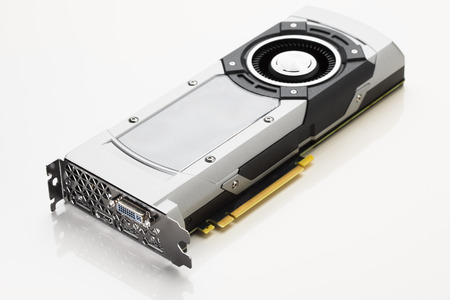
\includegraphics[width=0.5\linewidth]{fig/gpu.jpg}
\end{center}
\begin{center}
{\large Marc Fuentes - INRIA Pau\\ }
\end{center}
\end{frame}

%****************************************************************
% Xedea
%**************************************************************

\begin{frame}{Plan}
\begin{itemize}[<+->]
\item Prolégomenes (parallèlisme, mémoire, cache et Cie)
\item exemple d'introduction
\item modèle d'execution d'un GPU
\item accès mémoire et coalescence
\end{itemize}
\end{frame}

%****************************************************************
% Prolegomènes I
%****************************************************************
\begin{frame}
\frametitle{Parallèlisme}
\pause
différentes classifications du parallèlisme
\begin{itemize}[<+->]
  \item mémoire partagée / distribuée
    \begin{itemize}
      \item à mémoire partagée : OpenMP, fils d'éxecution (Threads), GPU 
      \item à mémoire distribuée : MPI, Coarrays Fortran, PGAS
    \end{itemize}
 \item gros grain / grain fin : taille des tâches
   \begin{itemize}
     \item gros grain : MPI, certains tâches en mémoire partagée
     \item grain fin : noyaux GPU s'executant sur beaucoup de cœurs
   \end{itemize}
 \item archi homogène / hétérogène 
   \begin{itemize}
     \item homogène : MPI, processeurs vectoriels
     \item hétérogène : accélérateur/hôte, processeur Cell (PS3)
   \end{itemize}
\end{itemize}
\pause
  \gezi La programmation sur GPU est {\it grosso modo } donc un parallèlisme à {\bf grain fin}, à mémoire {\bf partagée} tournant sur
  une architecture {\bf hétérogène}.
\end{frame}

%****************************************************************
% Prolègomène II
%****************************************************************
\begin{frame}{Mémoire et Cache}
\begin{itemize}[<+->]
  \item La rapidité d'execution d'un calcul dépend aussi de la «proximité» avec le CPU de l'élément de mémoire à traiter 
  \item[\gezi] les concepteurs de CPU ont crée des {\bf caches} pour stocker les valeurs mémoires les plus utilisées
  \begin{center}
    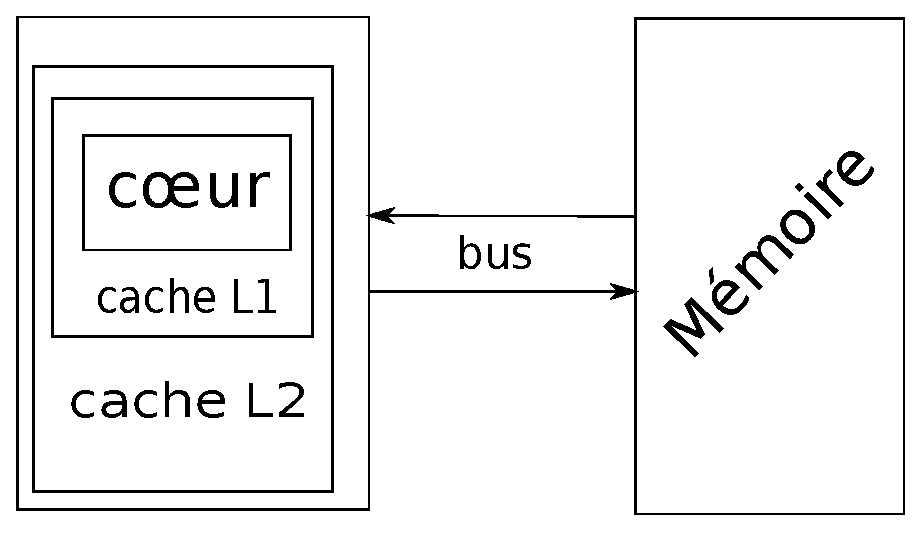
\includegraphics[width=0.7\linewidth]{fig/cpu_classique.eps}
  \end{center}
\end{itemize}
\end{frame}
%****************************************************************
% Prolegomenes III
%****************************************************************
\begin{frame}{Mémoire et Cache (II)}
\pause
  \begin{itemize}[<+->]
  \item ainsi la latence $l$ de l'emplacement mémoire auquel on accède  respecte
  $$l({\mbox{\scriptsize registre}}) \leqslant l(\mbox{\scriptsize cache L1}) \leqslant
    l(\mbox{\scriptsize cache L2}) \leqslant l(\mbox{\scriptsize mémoire globale}).$$
  \item ordres de grandeur des latences (core i7 Xeon E5500)
    \begin{tabular}{|l|c|c|}
    \hline
      type & nb cycles & latence (ns)  \\
    \hline
      cache L1  &  4 & 2 \\
      cache L2  &  10 & 5 \\
      cache L3 (non partagé) & 40 & 20  \\
      cache L3 (partagé) &  65 & 35  \\
      mémoire vive local & & 60 \\
      mémoire vive distante & & 100 \\
    \hline
    \end{tabular}
  \end{itemize}
\end{frame}
%%****************************************************************
%% Prolegomenes IV
%%****************************************************************
\begin{frame}{Cache : Succès et défauts}
\begin{itemize}[<+->]
 \item succès (hit): accès à un emplacement présent dans la ligne de cache 
 \item défaut (miss) : accès hors de la ligne de cache $\rightarrow$ il faut recharger entierement la ligne de cache!
 \item un code localisant ses accés dans le cache minimise les défauts de cache et tourne plus vite
 \item ex. double boucle en C sur les lignes (resp. colonnes en Fortran)
\end{itemize}
\pause
\begin{minipage}[c]{0.49\linewidth}
  \lstinputlisting[language=C]{code/loop_col.c}
\end{minipage}
\begin{minipage}[c]{0.49\linewidth}
    \begin{tabular}{|c|c|}
    \hline
     boucle ext. & tps(s)  \\
    \hline
      i (lignes) & 2.7s \\
      j (cols)  & 3.4s \\
    \hline
    \end{tabular}
\end{minipage}
\pause 
 $\Rightarrow$ raison d'être des biblios BLAS et LAPACK
\end{frame}
%%****************************************************************
%% Prolegomenes V
%%****************************************************************
\begin{frame}{Passage à l'échelle}
\begin{itemize}[<+->]
  \item fort (strong scalability)
    \begin{itemize} 
       \item loi d'Amdhal (pessimiste)
    \end{itemize}
  \item faible (weak scalability)
    \begin{itemize}
      \item loi
    \end{itemize}
\end{itemize}
\end{frame}
%%****************************************************************
%% Exemple introductif I
%%****************************************************************
\begin{frame}{Exemple d'introduction (I)}
\pause
\begin{itemize}[<+->]
 \item soit un programme calculant \texttt{tab[:]} $\leftarrow$ \texttt{tab[:] + 3}
\lstinputlisting{code/increment.c}
\item on souhaite paralléliser la boucle en ligne 6 à l'aide de CUDA
\end{itemize}
\end{frame}
%%****************************************************************
%% Exemple introductif II
%%****************************************************************
\begin{frame}{Exemple d'introduction (II) }
\pause
\begin{itemize}[<+->]
 \item on peut écrire le programme suivant
\lstinputlisting{code/incrementGPU.cu}
\item plus de boucle!
\item nouveaux mot-clefs : \texttt{\_\_global\_\_, threadIdx}
\item appel du noyau \texttt{increment<<<1,N>>>}
\item gestion de la mémoire : \texttt{cudaMemcpy, cudaMalloc, cudaFree}
\end{itemize}
\end{frame}
%****************************************************************
% Principe du //isme GPU
%****************************************************************
\begin{frame}{Exemple d'introduction (III)}
\pause
\begin{itemize}[<+->]
  \item boucle \textbf{for} $\rightarrow$ appel d'un {\bf thread}...
 \item executant le noyau \textbf{increment}
 \item pour chaque indice de boucle : \textbf{threadIdx.x }
 \item sur le tableau \textbf{tab\_d} alloué sur le GPU
 \item il faut copier \textbf{tab} sur le GPU et le rapatrier après calcul
\end{itemize}
\pause
\begin{center}
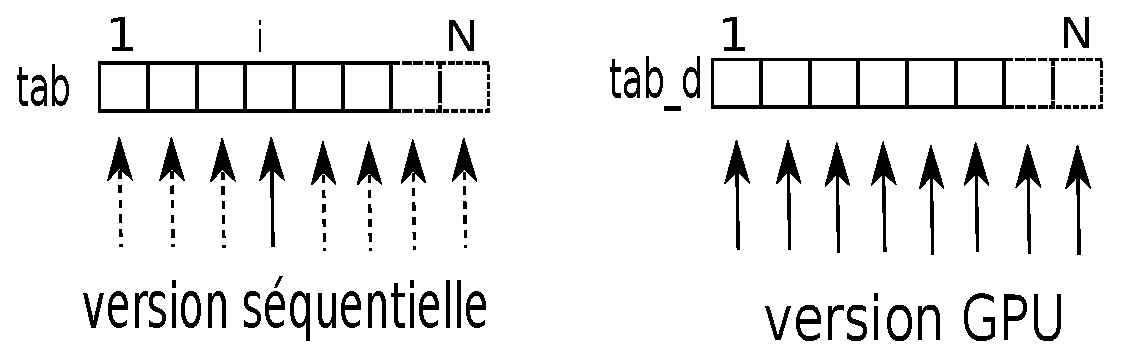
\includegraphics[width=0.9\linewidth]{fig/parallel.eps}
\end{center}
\end{frame}
%****************************************************************
% Déroulé classique d'un calcul
%****************************************************************
\begin{frame}{Déroulé typique d'un calcul}
\pause
  \begin{itemize}[<+->]
  \item un programme CUDA suit généralement les étapes suivantes 
\begin{enumerate}[<+->]
 \item allouer la mémoire sur le GPU : \texttt{cudaMalloc, cudaMallocPitch, cudaMalloc3D}
 \item copier depuis la mémoire globale vers le GPU : \texttt{cudaMemCpy($\cdots$,cudaMemcpyHostToDevice)}
 \item exécuter le noyau sur l'accélerateur : \texttt{myKernel<<<...,...>>>(...)}
 \item rapatrier les résultats en mémoire globale \texttt{cudaMemCpy($\cdots$,cudaMemcpyDeviceToHost)}
 \item visualiser les résultats
\end{enumerate}
\item Avant de poursuivre, nous avons besoin de comprendre le modèle d'exécution sur GPU
\end{itemize}
\end{frame}
%****************************************************************
% Modèle d'execution GPU I
%****************************************************************
\begin{frame}{modèle d'exécution du GPU}
  \begin{flushright}
    illustration sur un vieux Tesla
  \end{flushright}
\begin{minipage}[c]{0.49\linewidth}
\begin{itemize}
  \item multiprocesseur de flux (SM)
    \begin{itemize}
      \item groupe de 8 processeurs de flux (SP)
        \begin{itemize}
          \item partage de mémoire locale
          \item synchronisation
        \end{itemize}
    \end{itemize}
  \item processeur de flux (SP) : 
    \begin{itemize}
    \item 64KB de registres, 
    \item {\bf threads} : ensemble de registres
    \begin{itemize}
      \item création/destruction gratuites
    \end{itemize}
  \item exécution entrelacée de {\em threads} matériels : jusqu'à 128 par SP
    \end{itemize}
\end{itemize}
\end{minipage}
\begin{minipage}[c]{0.49\linewidth}
\begin{center}
  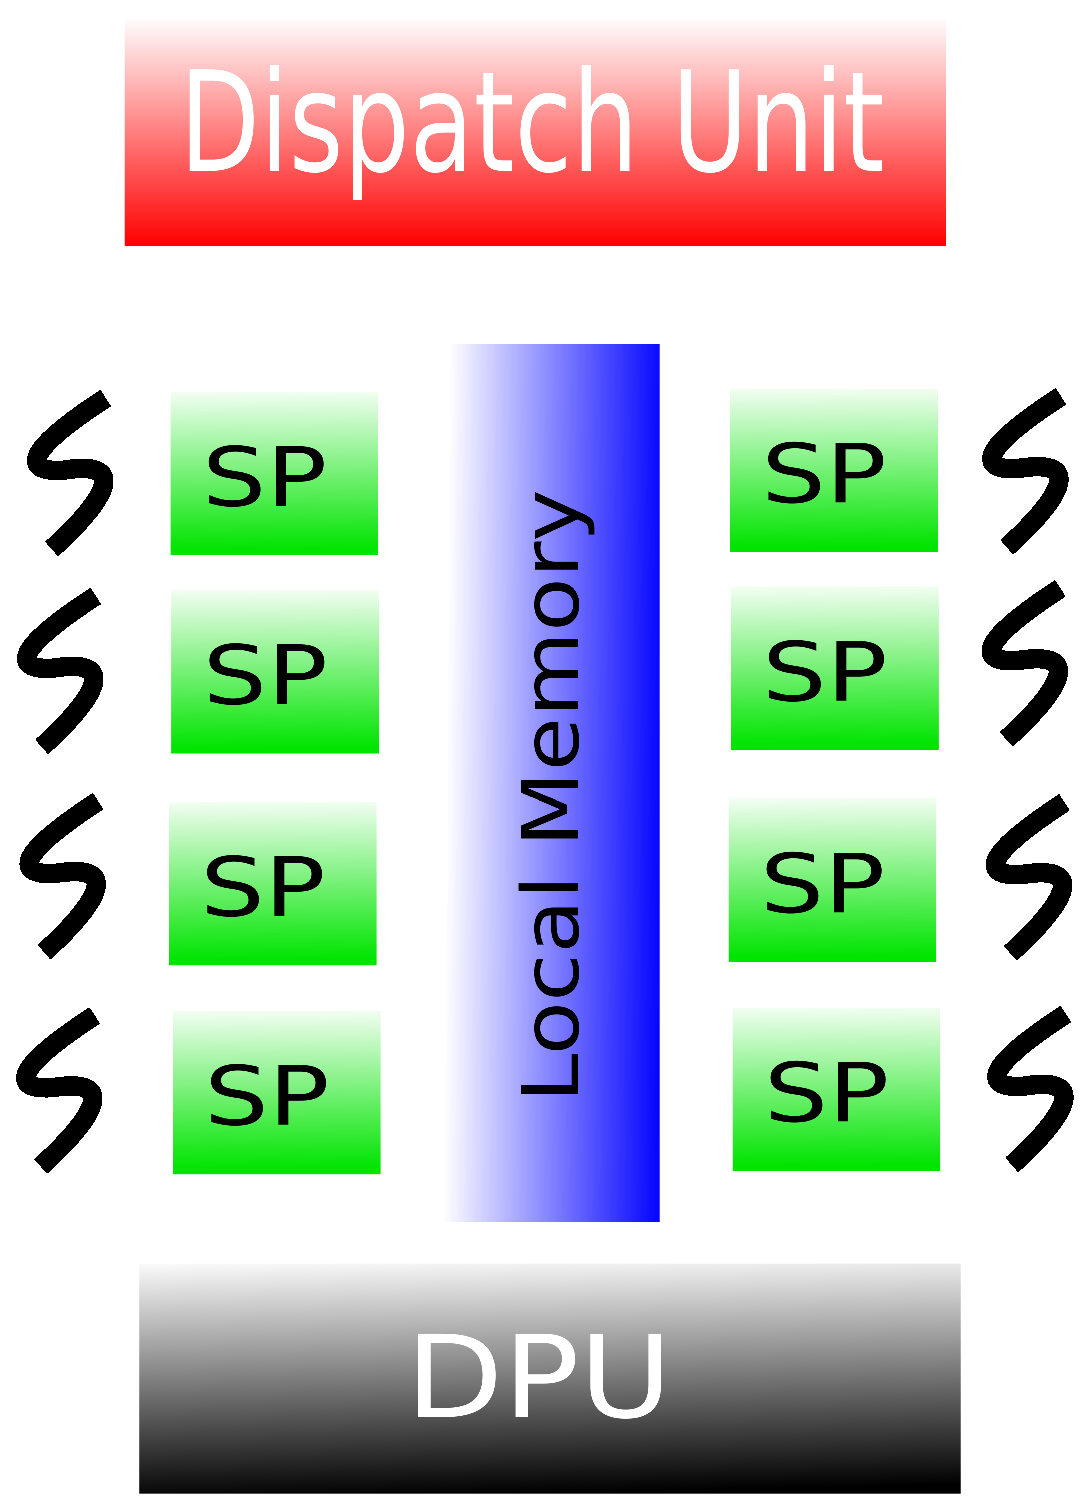
\includegraphics[width=0.6\linewidth]{fig/GPUArchiThread.eps}
\end{center}
\end{minipage}
\end{frame}
%****************************************************************
% Modèle d'execution GPU II
%****************************************************************
\begin{frame}{modèle d'exécution du GPU}
  \begin{flushright}
    illustration sur un vieux Tesla
  \end{flushright}
\begin{minipage}[c]{0.49\linewidth}
\begin{itemize}
  \item 1 seule unité d'envoi d'instruction par multiprocesseur de flux
    \begin{itemize}
      \item tous les SP executent la même instruction au même cycle d'horloge
        \begin{itemize}
          \item sur des données différentes (SIMD)
        \end{itemize}
    \end{itemize}
  \item l'unité d'envoi prend 4 cycles pour récupérer et décoder les instructions
    \begin{itemize}
      \item 4 groupes de 8 {\bf threads} planifiés / ligne
    executant la même instruction
      \item changement de contexte gratuit !
    \end{itemize}
\end{itemize}
\end{minipage}
\begin{minipage}[c]{0.49\linewidth}
\begin{center}
  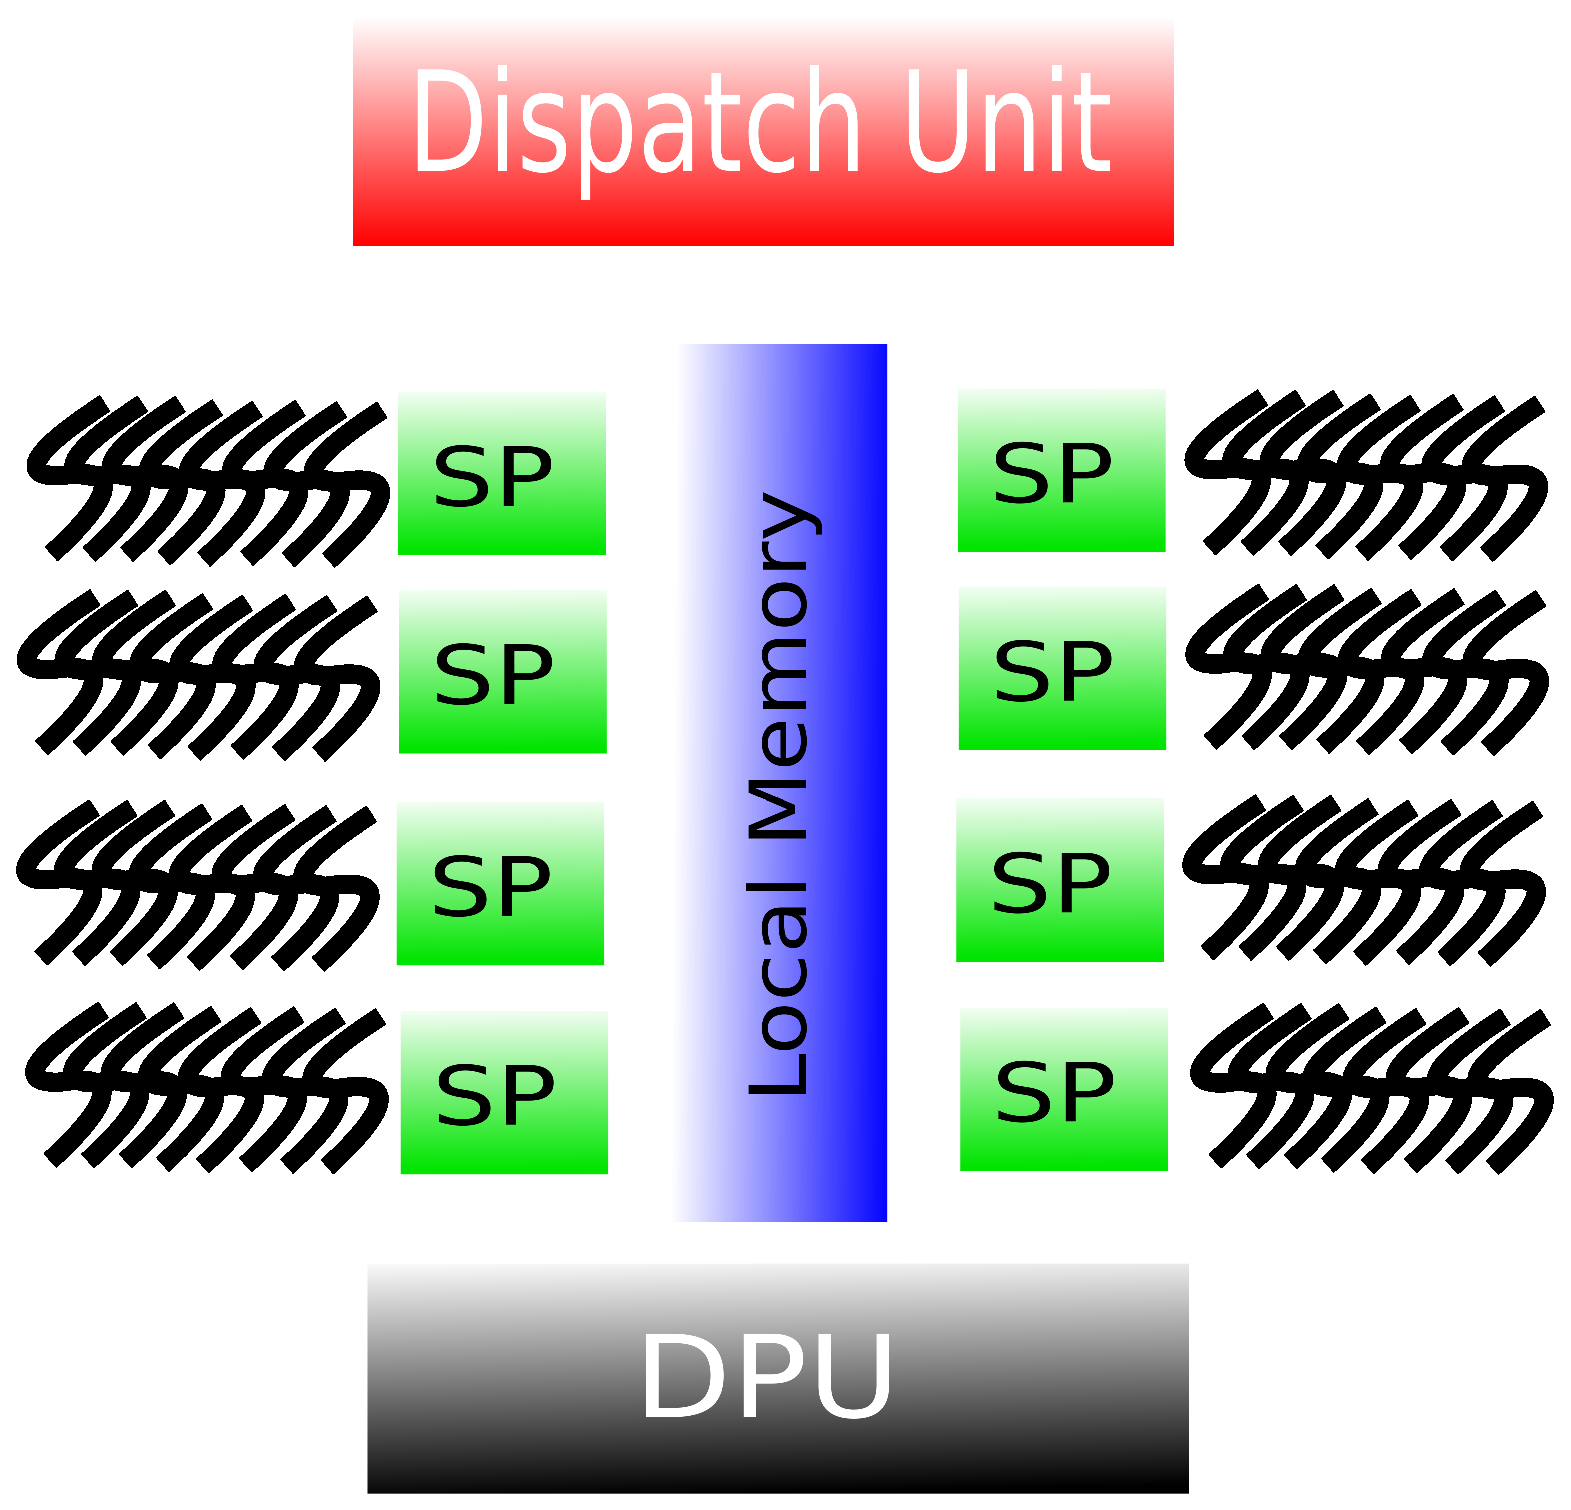
\includegraphics[width=0.9\linewidth]{fig/GPUArchi8Thread.eps}
\end{center}
\end{minipage}
\end{frame}
%****************************************************************
% Modèle d'execution GPU III
%****************************************************************
\begin{frame}{modèle d'exécution du GPU}
  \begin{flushright}
    {\bf warps } et {\bf demi-warps}
  \end{flushright}
\begin{minipage}[c]{0.49\linewidth}
\begin{itemize}
  \item les {\bf threads} sont implicitement groupés en {\bf warps}
    \begin{itemize}
      \item un {\bf warp} (chaîne) = 32 threads 
      \item tous les threads d'une même chaîne executent la même instruction au même cycle logique
        \begin{itemize}
          \item pas de divergence
        \end{itemize}
    \end{itemize}
  \item charger des données depuis la mémoire globale est coûteux
    \begin{itemize}
      \item plus de 4 threads nécessaire par SP
      \item 128 permettent de recouvrir la latence mémoire
    \end{itemize}
\end{itemize}
\end{minipage}
\begin{minipage}[c]{0.49\linewidth}
\begin{center}
  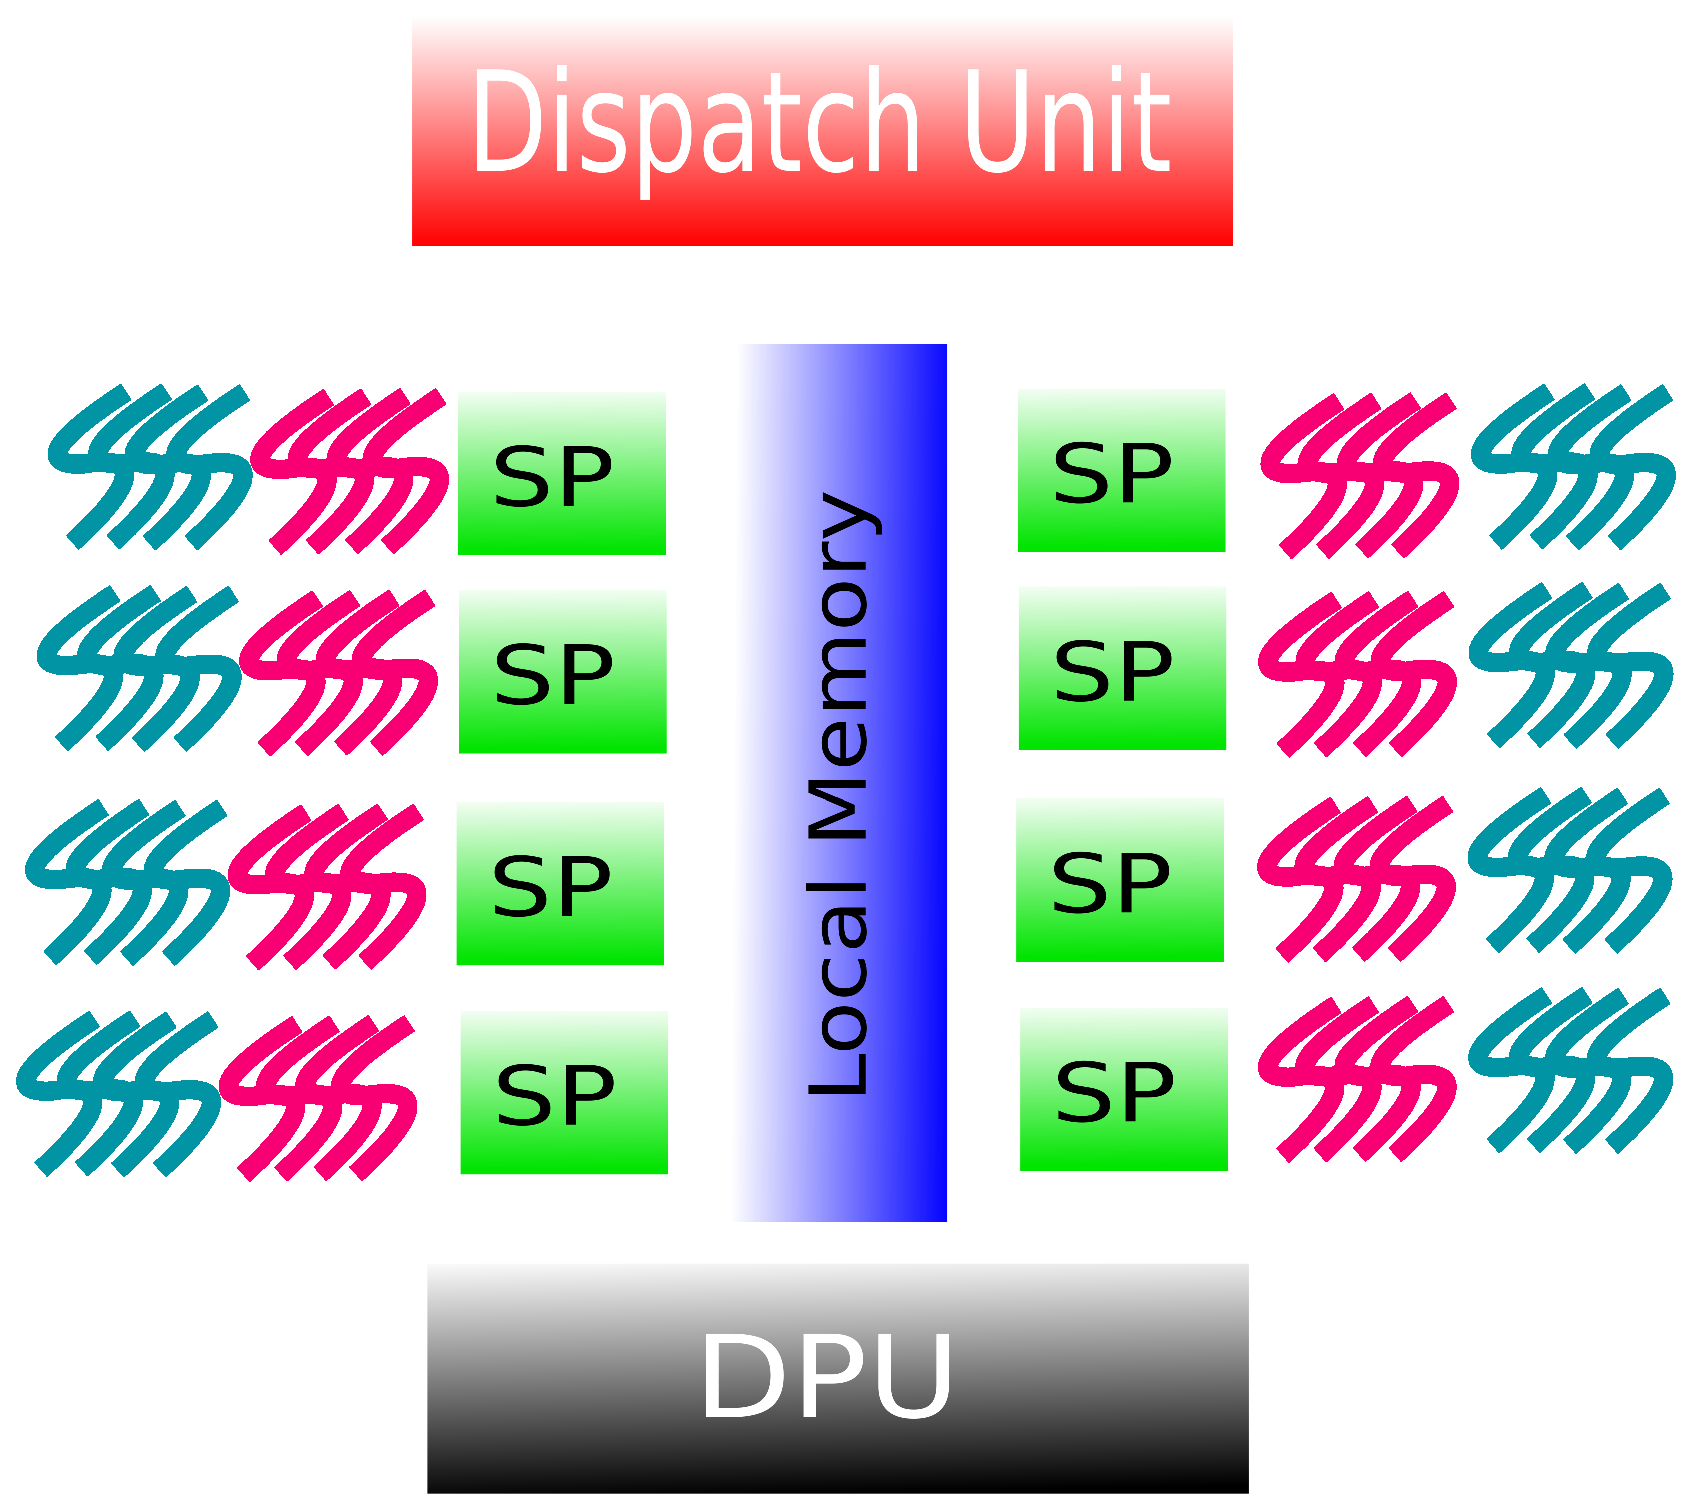
\includegraphics[width=0.9\linewidth]{fig/GPUArchi8ThreadDiv.eps}
\end{center}
\end{minipage}
\end{frame}
%****************************************************************
% Modèle d'execution GPU IV
%****************************************************************
\begin{frame}{modèle d'exécution du GPU}
  \begin{flushright}
   illustration avec un K40M
  \end{flushright}
\begin{minipage}[c]{0.49\linewidth}
  \begin{itemize}[<+->]
    \item GPU = ensemble de multiprocesseurs de flux (SM) partageant une mémoire global (DRAM)
    \item Tesla K40M : 
      \begin{itemize}
        \item 15 SM, 192 SP / SM $\Rightarrow$ 2880 SP
        \item 2048 threads max / SM $\Rightarrow$ 30.720 threads
      \end{itemize}
    \item threads «speciaux»
      \begin{itemize}
        \item parallélisme de données respectant des motifs d'accès réguliers
      \end{itemize}
  \end{itemize}
\end{minipage}
\begin{minipage}[c]{0.49\linewidth}
\begin{center}
  \rotatebox{90}{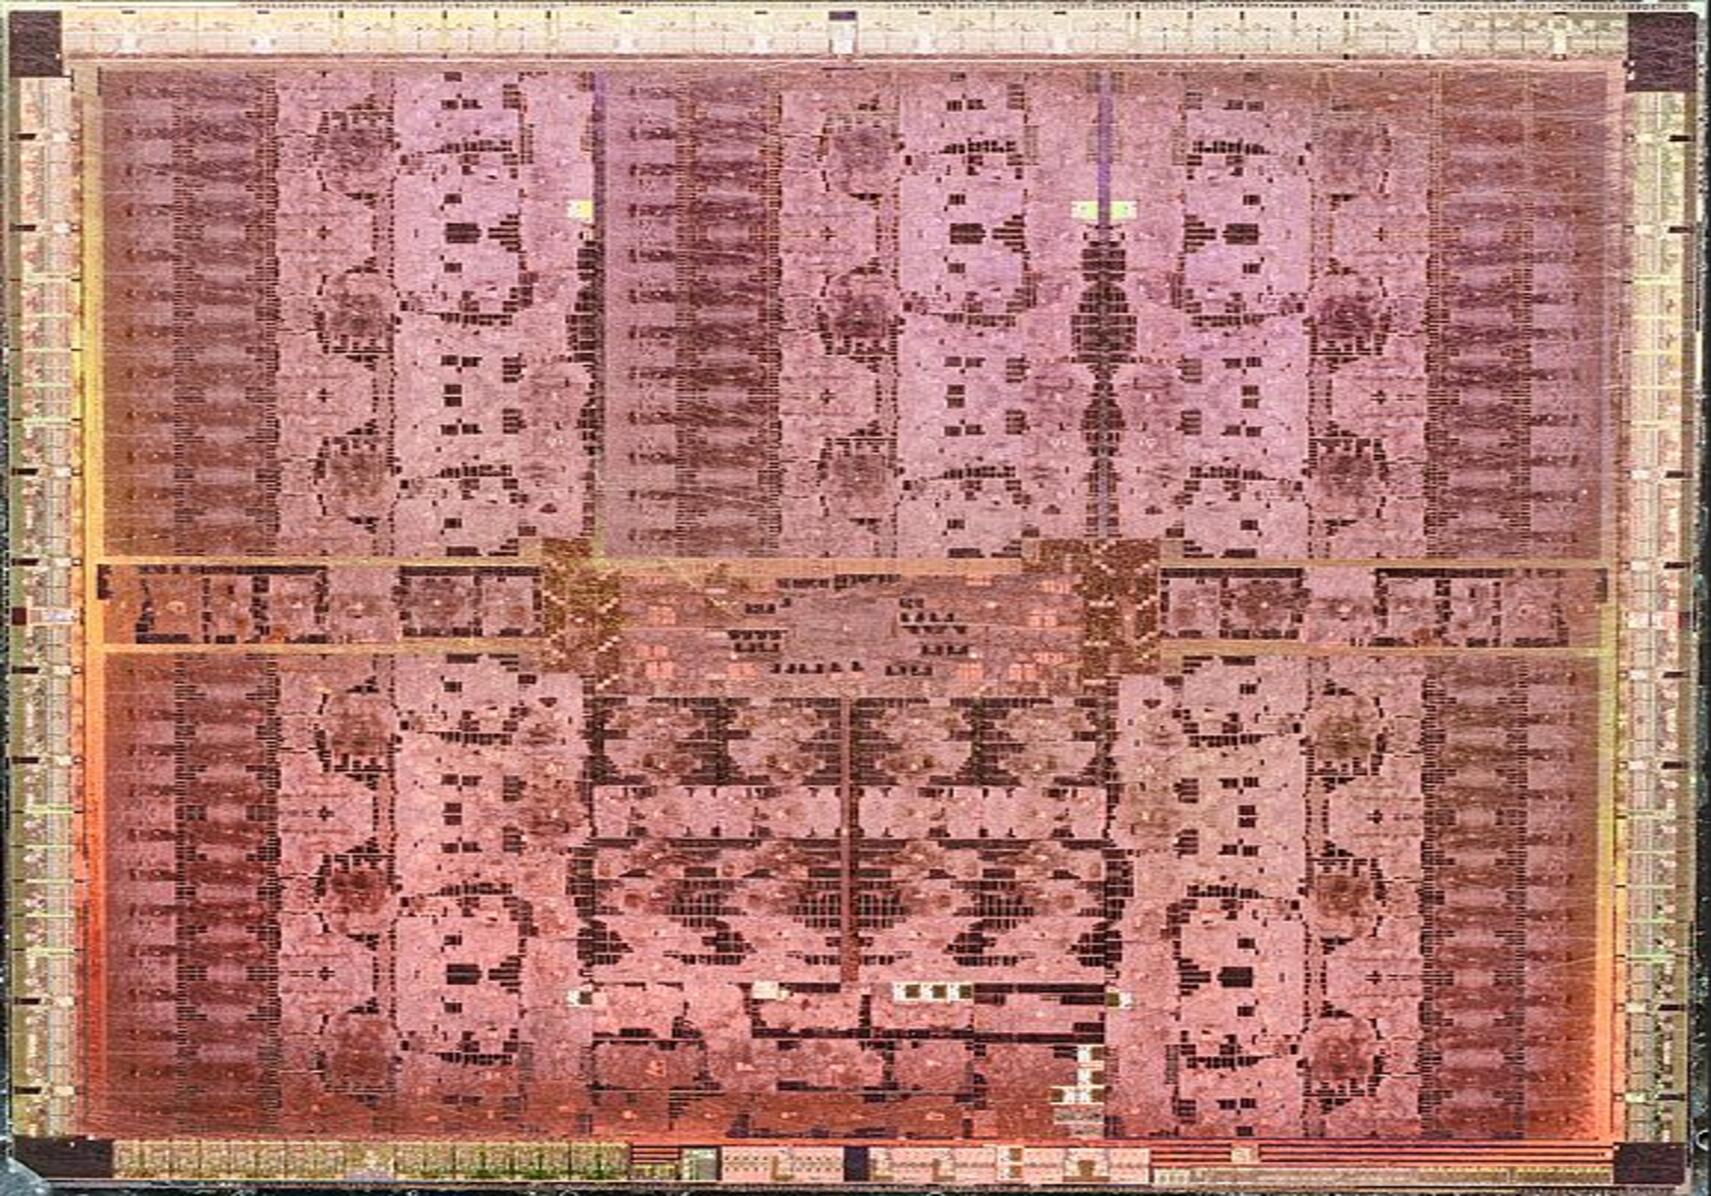
\includegraphics[width=0.9\linewidth]{fig/kepler.jpg}}
\end{center}
\end{minipage}
\end{frame}
%****************************************************************
% Organisation des threads
%****************************************************************
\begin{frame}{modèle d'exécution du GPU}
 \pause
 \begin{minipage}[c]{0.49\linewidth}
  \begin{itemize}[<+->]
    \item un K40M a $\approx$ 30K threads $\Rightarrow$ Que faire si $N \geq 30K$ ?
    \item Découpage des données en {\em blocs } et en {\em grille}
    \item organisation 1D, 2D ou 3D
      \begin{itemize}
        \item 15 SM, 192 SP / SM $\Rightarrow$ 2880 SP
        \item 2048 threads max / SM $\Rightarrow$ 30,720 threads
      \end{itemize}
    \item threads «speciaux»
      \begin{itemize}
        \item parallélisme de données respectant des motifs d'accès réguliers
      \end{itemize}
  \end{itemize}
\end{minipage}
\begin{minipage}[c]{0.49\linewidth}
\begin{center}
  \rotatebox{90}{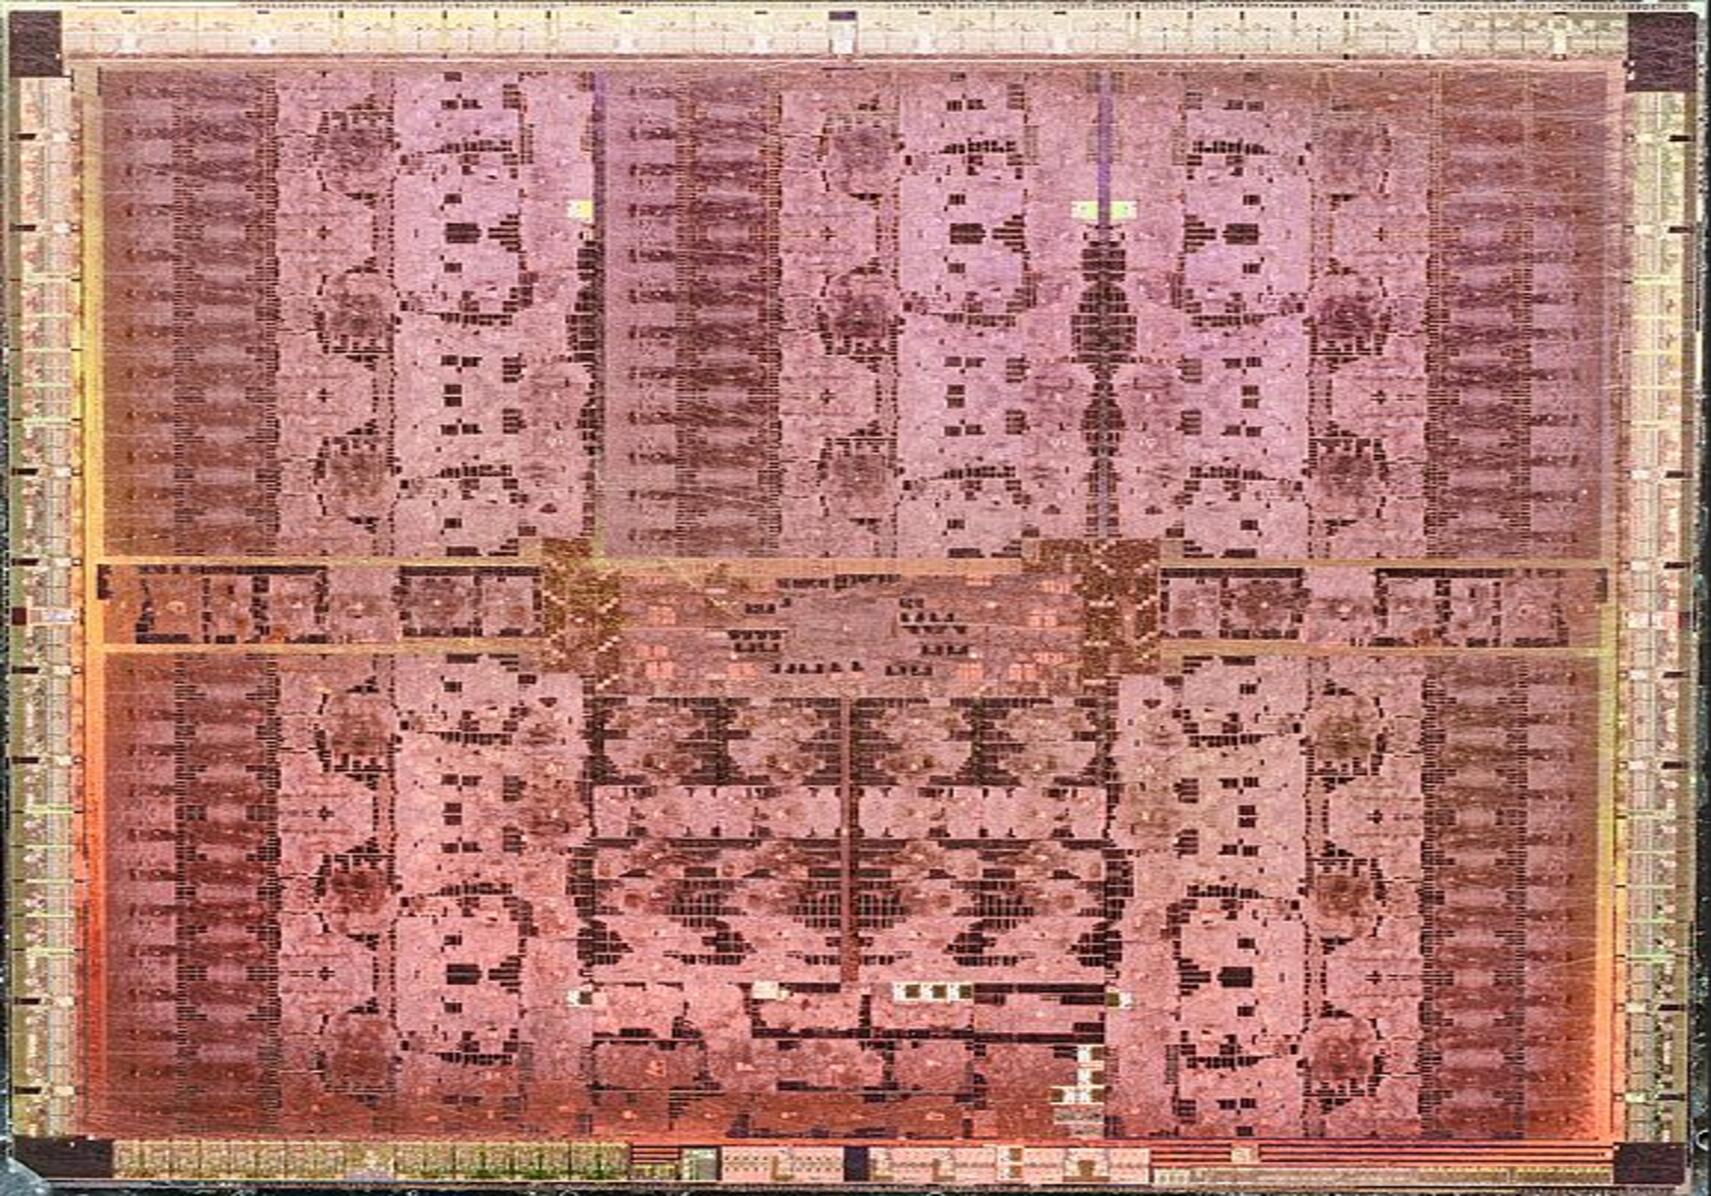
\includegraphics[width=0.9\linewidth]{fig/kepler.jpg}}
\end{center}
\end{minipage}
\end{frame}
%****************************************************************
% References
%****************************************************************
\begin{frame}{Références}
\begin{itemize}[<+->]
  \item Programming GPU Accelerators with OpenCL, R. Namyst, P.-A. Wacrenier \href{https://raymond-namyst.emi.u-bordeaux.fr/ens/pap/PAP-GPU.pdf}{\beamergotobutton{Pdf}}
  \item Cuda Fortran for Scientists and Engineers, G. Ruetsch, M. Fatica
  \item Understanding Latency Hiding on GPUs, V. Volkov
  \item CUDA Basics, S. Vialle \href{http://www.metz.supelec.fr/metz/personnel/vialle/course/PPS-5A-GPGPU/notes-de-cours-specifiques/PPS-GPU-02-CUDA-Basics-2spp.pdf}{\beamergotobutton{pdf}}
\end{itemize}
\end{frame}
\end{document}
